%%=========================================
\chapter{Characterisation Methods}\label{ch:methods}
%\todo{Må skrive om denne introduksjonen.}
%The surface layer of solids and liquids are different from the bulk matter. This can be a  different chemical composition, a different structure, or both. The surface layer can be defined as a small number of atomic layers that separate the solid from the surrounding world, where the bulk properties are no longer sufficient to describe its properties \citep{luth2010solid}. Hence, in order to describe the physical and chemical properties of a material, it is important to have methods that can characterise the surface layer. 

In order to describe the physical and chemical properties of a material, it is important to have methods that can characterise the surface layer. In this chapter, a description of the characterisation methods used to characterise the surface of the substrates is presented.\todo{Skriv kort hvilke teknikker som er brukt til hva.  Motiver leseren for hvorfor akkurat de valgte teknikkene blir presentert.}


%%=========================================
\section{Optical Microscopy}

The optical microscope uses visible light and optical lenses to magnify images of small features. There are different illumination techniques that can be used to increase the contrast from the sample. One of these techniques is bright field microscopy, where the scattered beam is excluded from the image and the contrast in the image comes from the absorption of light in the sample. A complementary technique is dark field microscopy, in which the unscattered beam is excluded and it is the scattered light that forms the image. A third optical microscopy technique used to enhance the contrast, is Nomarski microscopy, which utilises the optical path length of the sample to see otherwise invisible features.

Even if all optical aberrations in the lens system are assumed to be negligible, i.e. a perfect lens, there will be a limit to how small details that can be resolved due to interference and diffraction of the light that passes through the system. Resolution is defined as the minimum distance between two points at which they can be distinguished. For two point sources surrounded by Airy discs of diffracted light, this minimum distance is at which the principal maximum of one source coincides with the first minimum of the second source. If the sources have equal wavelength, then the Airy discs have the same radius and this minimum distance is equal to the radius of one Airy disc, measured from the principal maximum to the first minimum intensity. This is called the Rayleigh criterion \citep{rayleigh1879investigations, rayleigh1880investigations}. The corresponding angle of resolution $\theta$ is given by
\begin{equation}\label{eq:rayleigh}
\theta = \SI{1.22}{}\frac{\lambda}{D},
\end{equation}
where $\lambda$ is the wavelength of the light and $D$ is the diameter of the aperture. $\theta$ may be converted into spatial resolution $d$ by multiplying Eq.~\eqref{eq:rayleigh} with the distance to the object. For a microscope this distance is approximately the focal length $f$ of the objective. Then Eq.~\eqref{eq:rayleigh} becomes
\begin{equation}\label{eq:rayleigh2}
d = \SI{1.22}{}\frac{\lambda f}{D}.
\end{equation}

The term numerical aperture is used in microscopy to describe the acceptance cone of an objective. Numerical aperture is defined as
\[\text{NA}=n\sin\theta_\text{cone},\]
where $n$ is the refractive index and $\theta_\text{cone}$ is the half-angle of the maximum cone of light that can enter or exit the lens. Using geometrical considerations and the small angle approximation, the numerical aperture can be expressed as
\begin{equation}\label{eq:numap}
\text{NA} = n\frac{D/2}{f}.
\end{equation}
Inserting Eq.~\eqref{eq:numap} into Eq.~\eqref{eq:rayleigh2} gives
\begin{equation}\label{eq:rayleigh3}
d = \SI{0.61}{}\frac{n\lambda}{\text{NA}}.
\end{equation}

Eq.~\eqref{eq:rayleigh3} shows that there is a linear relation between resolution and the wavelength of the incoming light. If the wavelength is reduced, it becomes possible to resolve smaller details. For an optical microscope $\text{NA}$ is approximately 1 and the refractive index in air is approximately 1. Then, for visible light, i.e. wavelengths in the range \SI{400}{\nano\metre} to \SI{680}{\nano\metre}, it would be possible to achieve a resolution of \SI{244}{\nano\metre} to \SI{415}{\nano\metre} with an optical microscope. Since the spatial resolution is proportional to $\lambda$, blue light can be focused to a smaller spot than red light due to its shorter wavelength.
%%=========================================
\section{Near-Infrared Transmission Microscopy}
%
Materials that are transparent to infrared radiation can be investigated using \acf{nirts}. This is a technique which images \ac{ir} radiation that is transmitted through a sample. The contrast in the image is formed from the interaction of the beam through the sample. E.g. precipitates consist of another material with different optical properties than the sample matrix and may not be transparent to \ac{ir} radiation, and hence, appear as dark spots in the resulting image.

The light bulb used to illuminate the sample can be considered a blackbody. The photon radiance from a perfect blackbody is given by Planck's law of blackbody radiation. The number of photons emitted per unit wavelength $\lambda$ per second per steradian from one square meter of a perfect blackbody at temperature $T$ is \citep{liboff2003introductory}
\begin{equation}\label{eq:planck-law}
L_\lambda (T) = \frac{2c}{\lambda^4}\parentheses{\mathrm{e}^{\frac{hc}{kT\lambda}}-1}^{-1},
\end{equation}
where $h=\SI{6.63e-34}{\joule\second}$ is Planck's constant, $c=\SI{3.00e8}{\metre\second^{-1}}$ is the speed of light and $k=\SI{1.38e-23}{\joule\kelvin^{-1}}$ is Boltzmann's constant.

The highest spatial resolution of an infrared microscope is defined by the diffraction limit of the radiation, see Eq.~\eqref{eq:rayleigh3}. Over the near-infrared region the wavelengths vary between \SI{750}{\nano\metre} and \SI{1.4}{\micro\metre}. Hence, if a microscope with ideal numerical aperture of 1 is used in air, where the refractive index is approximately 1, then the maximum spatial resolution will be between \SI{550}{\nano\metre} and \SI{850}{\nano\metre}.

%%=========================================
\section{Scanning Electron Microscopy}
\Acf{sem} is a technique that is used to study materials at greater magnification than with optical microscopy. A point resolution of less than \SI{1}{\nano\metre} can be achieved using the \ac{sem} \citep{goldstein2012scanning}. The \ac{sem} utilises electrons and magnetic lenses in the place of photons and optical lenses in optical microscopy. Even though the image is created in a different way than in the optical microscope, the maximum resolution is still limited by the wavelength of the particle used, which in this case is the electron. 

The wavelength of an electron is given by the de Broglie relationship \citep{de1924recherches}
\begin{equation}
\label{eq:debroglie}
\lambda = \frac{h}{p},
\end{equation}
where $h=\SI{6.63e-34}{\metre^2\kilo\gram\second^{-1}}$ is Planck's constant and $p$ is the momentum of the electron. The momentum of the electron can be calculated using the energy-momentum relation
\begin{equation}
\label{eq:energy-momentum_relation}
E^2 = (pc)^2 + (m_0c^2)^2,
\end{equation}
where $E$ is the total energy of the electron, $c$ is the speed of light, and $m_0$ is the electron's rest mass. The total energy is the sum of the rest mass energy $m_0c^2$ and the kinetic energy $E_\mathrm{k}$. When an electron at rest is accelerated through a potential difference $U$, its kinetic energy  will become equal to the energy of the field $E_\textrm{k} = e U$, where $e=\SI{1.60e-19}{\coulomb}$ is the elementary charge. This gives that the total energy of the electron is
\begin{equation}
\label{eq:electron_energy}
E = m_0c^2 + eU.
\end{equation}

An expression for the momentum of the electron is obtained by inserting Eq.~\eqref{eq:electron_energy} into Eq.~\eqref{eq:energy-momentum_relation}
\begin{equation}
\label{eq:electron_momentum}
pc = \sqrt{(eU)^2 + 2m_0eUc^2}.
\end{equation}

When inserting Eq.~\ref{eq:electron_momentum} into Eq.~\ref{eq:debroglie}, the de Broglie wavelength can be calculated from the known variables $h$, $m_0$, $e$, $U$ and $c$
\begin{equation}
\label{eq:electron_wavelength}
\lambda = \frac{h}{\sqrt{2m_0eU\brackets{1 + eU/(2m_0c^2)}}}.
\end{equation}

For a \SI{1.00}{\kilo\volt} accelerating potential, the electron wavelength is \SI{3.88e-2}{\nano\metre}, while for a \SI{25.0}{\kilo\volt} accelerating potential, the electron wavelength is \SI{7.66e-3}{\nano\metre}, according to Eq.~\ref{eq:electron_wavelength}. These small wavelengths allow the \ac{sem} to achieve high resolution images. The electromagnetic lenses, which are needed to focus the electron beam, limit $\theta_\text{cone}$ to \SI{e-2}{\radian}. Therefore, the diffraction limit, as given by Eq.~\eqref{eq:rayleigh3}, is \SI{2.37}{\nano\metre} and \SI{0.469}{\nano\metre} for accelerating voltages of \SI{1.00}{\kilo\volt} and \SI{25.0}{\kilo\volt} respectively. This is the theoretical limit, but the real obtainable resolution is lower due to spherical aberration, chromatic aberration, astigmatism, and distortion \citep{brandon2013microstructural}.

The \ac{sem} produces images by raster-scanning a focused beam of electrons across the sample and plotting the intensity of different signals versus beam position. During the interaction with the sample, the incoming \acp{pe} are the source to emitted \acp{se}, \acp{bse}, \acp{ae}, bremsstrahlung, and characteristic X-rays. 

\Acp{se} are valence and conduction electrons emitted by atoms excited by the incident electron beam, see Fig.~\ref{fig:sem_se}. They have low energy (\SI{<50}{\electronvolt}) and emerge from very close to the sample surface, i.e. from a small interaction volume, which gives the possibility of high-resolution images. \Acp{bse} are incident electrons that scatter from the atomic nuclei and come back out of the sample, see Fig.~\ref{fig:sem_bse}. Larger atoms deflect more electrons, resulting in a larger signal at the detector. \Acp{bse} can emerge from deeper into the sample due to their high energy, i.e. from a greater interaction volume, which can result in a poorer resolution than secondary electron images. \Ac{se} is generally the preferred signal when imaging sample topography in \ac{sem} \citep{sealy2000mechanism}. The brightness of the signal increases with the number of detected \acp{se}. 

When an electron from an inner shell is emitted and leaves a vacancy, an electron from a higher energy shell can fall down and fill the vacant energy level, resulting in excess energy. This energy can be released in the form of an emitted photon, i.e. an X-ray, see Fig.~\ref{fig:sem_x-ray}, or it can be transferred to another electron in an outer shell, which is then emitted from the atom and takes the excess energy with it, see Fig.~\ref{fig:sem_auger}. The emitted electron is called \iacl{ae}.

\begin{figure}[htbp]
    \centering
    \mySubfigure{0.48\linewidth}{sem_se.png}[fig:sem_se]
    \hfill
    \mySubfigure{0.48\linewidth}{sem_bse.png}[fig:sem_bse]
    \par\bigskip
    \mySubfigure{0.48\linewidth}{sem_x-ray.png}[fig:sem_x-ray]
    \hfill
    \mySubfigure{0.48\linewidth}{sem_auger.png}[fig:sem_auger]
    \caption[Illustration of the various modes of electron or X-ray emission from an incident electron.]{Illustration of the various modes of electron or X-ray emission from an incident \acf{pe}: \subref{fig:sem_se} \Iacf{se} is emitted when the atom is excited by the incident electron beam; \subref{fig:sem_bse} \iacf{bse} is an incident electron that scatter from the atomic nuclei and come back out of the sample; and \subref{fig:sem_x-ray} and \subref{fig:sem_auger} are the emission of an X-ray and an electron, respectively, to release excess energy after an electron from a higher energy shell falls down and fills a vacant energy level. The vacancy is formed by the emission of a secondary electron, see Fig.~\subref{fig:sem_se}. The filled black circle represents the atomic nucleus, the circle with a minus sign represents an electron, the grey circle represents a vacant energy level, and the curly orange arrow represents the emission of an X-ray \citep[Adapted from][]{goldstein2012scanning}.}
    \label{fig:sem_ill}
\end{figure}


%%=========================================
\section{Energy Dispersive X-ray Spectroscopy}\label{sec:eds}
\Acf{eds} is a technique used for the elemental analysis or chemical characterisation of a sample. Characteristic X-rays are produced during the interaction of the incident electron beam with the sample and can be detected using \ac{eds}. A characteristic X-ray is emitted when an incident electron kicks out an electron from an inner shell in an atom, and an electron from a higher-energy shell falls down to the lower-energy shell and releases the excess energy by emitting a photon. These excitations and de-excitations occur between discrete energy levels characteristic of the element. The characteristic X-rays form a spectrum that is unique for the elements involved, just like a fingerprint. Hence, \ac{eds} can be used to determine the elemental composition of the material by evaluating the characteristic energy lines. 

In addition to the characteristic X-rays, bremsstrahlung is produced. This is electromagnetic radiation produced by the deceleration of a charged particle, i.e. the electron, when it is deflected by another charged particle, i.e. the atomic nucleus. The particle loses kinetic energy and the excess energy is transferred away as a photon.

A summary of the interaction volumes of the various modes of electron or X-ray emission from an incident electron can be seen in Fig.~\ref{fig:sem_interaction_volume}. The interaction volume increases with increasing electron energy, i.e. increasing accelerating voltage, and decreases with increasing average atomic number of the sample \citep{goldstein2012scanning}. Therefore, it is necessary to work at as low an accelerating voltage as possible taking into account what elements are present and which X-ray lines are needed.%Therefore, it is necessary to use low accelerating voltages when obtaining \ac{sem} images, i.e. \SIrange{0.5}{5}{\kilo\volt}, to prevent a large interaction volume and get generation of secondary electrons from the feature of interest \citep{}.

\begin{figure}[htbp]
    \centering
    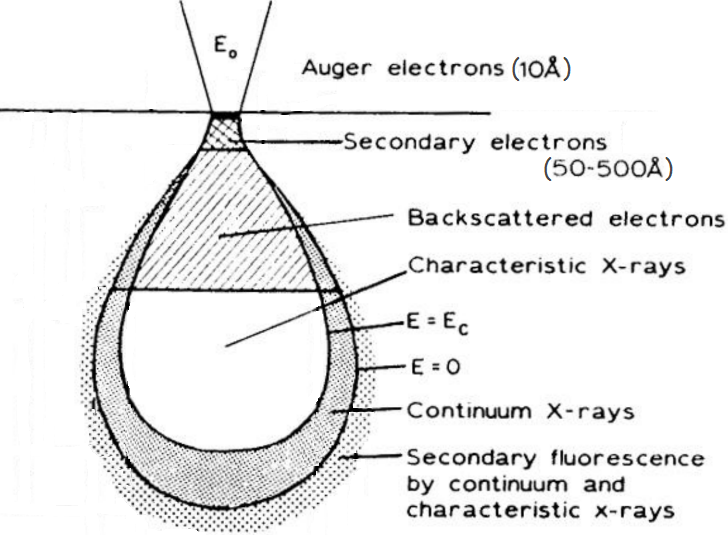
\includegraphics[width=0.6\linewidth]{sem_interaction_volume.png}
    \caption[Range and spatial resolutions of backscattered electrons, secondary electron, X-rays, and Auger electrons produced from a SEM.]{Range and spatial resolutions of backscattered electrons, secondary electron, X-rays, and Auger electrons produced from a scanning electron microscope. The outline of the volume of characteristic X-ray production is defined by the case where the electron energy $E$ is just sufficient to produce X-rays requiring the critical energy $E_c$, which varies with the X-ray of interest. The outline of the volume of continuum X-ray (bremsstrahlung) production is where $E$ is zero and cannot be decelerated any longer \citep[Reprinted from][]{goldstein2012scanning}.}
    \label{fig:sem_interaction_volume}
\end{figure}

Absolute concentration values of the elements are obtained using P/B-ZAF analysis. The local peak to bremsstrahlung background ratios (P/B) are input to a modified ZAF matrix correction, which relate the recorded spectrum to the primary rate of X-ray generation. This is done mainly based on analytical expressions to correct for atomic number depended X-ray yield (Z), self-absorption (A), and secondary fluorescence enhancement (F) \citep{quantax2008microanalysis}. Since P/B-ZAF do not use explicit or implicit standards in the calculation of concentrations, it is called a true standardless method.%, and self-calibrating.

 %using the P/B-ZAF algorithm the characteristic X-ray intensities (i.e. the net peak areas) are calculated in relation to the mean level of the simultaneously recorded bremsstrahlung background

%%=========================================
\section{X-ray Photoelectron Spectroscopy}\label{sec:xps}
\Acf{xps} is used to find the elemental composition of the outer surface of a solid (\SI{\sim 100}{\angstrom}). In addition, \ac{xps} can be used to get information about the chemical binding state of the detected elements.

\Ac{xps} is based on the emission and detection of photoelectrons. The sample is bombarded with a beam of X-ray photons of energy $E_\text{photon}$. If $E_\text{photon}$ is sufficiently large, i.e. greater than the binding energy of an electron $E_\text{binding}$, it can kick out the electron from an inner shell in an atom. If the photoelectron is close to the surface, it can be emitted from the sample to the vacuum outside, with a kinetic energy given by
\begin{equation}
    E_\text{kinetic} = E_\text{photon} - E_\text{binding} - \phi,
\end{equation}
where $\phi$ is the work function that accounts for the loss of energy as the electron leaves the sample and is absorbed by the detector. The detector measures the kinetic energy of the emitted photoelectron. Since the electron binding energies are at discrete energy levels, and these are element and chemical-bonding state dependent, a spectrum of the number of emitted electrons as a function of binding energy reveals which elements are present in the sample and their chemical-bonding state.

The mean free path of the photoelectrons in a material is on the order of \SI{20}{\angstrom} \citep{tanuma1991calculations}. Hence, only electrons emitted from atoms within a few mean free paths from the surface, i.e. \SI{80}{\angstrom}, are able to escape the material without loss of energy and be detected as peaks in the spectra. This makes \ac{xps} a surface sensitive technique that can tell us about the outermost layer of the sample. The electrons that are scattered inelastically before leaving the sample form the continuous background of the spectrum.

Quantification of the composition in the sample can be made by finding the ratios of the peak areas for the elements found in the sample. The atomic fraction of element $A$ in a homogeneous solid is estimated to be \citep{moulder2000handbook}
\begin{equation}\label{eq:xps_concentration}
    C_\mathrm{A} = \frac{I_\mathrm{A}/S_\mathrm{A}}{\sum_i I_i/S_i},
\end{equation}
where $I_\mathrm{A}$ is the measured peak area for element A, and analogously for $I_i$; and $S_\mathrm{A}$ is the sensitivity factor of element A, and analogously for $S_i$. The sensitivity factors take into account parameters that affect the intensity of the element, such as the distinctive cross-sections and densities of the different elements, and normalise these to that of the most intense peak. %the beam experience as it collide with the elements in the sample, that increase or decrease the probabilities for exciting a photoelectron.
% where $I_\mathrm{A}/I_i$ is the measured peak area for element A/$i$ and $S_\mathrm{A}/S_i$ is the sensitivity factor of element A/$i$.

A simple model for an abrupt uniform layer L on a bulk material B is used to estimate the thickness $d$ of a layer. The ratio between the signal from the layer and the signal from the bulk as a function of $d$ is given by \citep{briggs1990practical} 
\begin{equation}\label{eq:signal_ratio}
    R(d) = \parentheses{\frac{a_\mathrm{B}}{a_\mathrm{L}}}^3 \frac{\lambda_\mathrm{LL}}{\lambda_\mathrm{BB}} \frac{1-\exp{\parentheses{-\frac{d}{\lambda_\mathrm{LL}\cos\theta}}}}{\exp{\parentheses{-\frac{d}{\lambda_\mathrm{BL}\cos\theta}}}},
\end{equation}
where $a_\mathrm{B}$ is the atomic size of material B, and analogously for $a_\mathrm{L}$; and $\lambda_\mathrm{BL}$ is the inelastic mean free paths of photoelectrons emitted from material B in layer L, and analogously for $\lambda_\mathrm{BB}$ and $\lambda_\mathrm{LL}$. The atomic size is derived from $1000\rho_\mathrm{M}N a_\mathrm{M}^3 = A_\mathrm{M}$, where $\rho_\mathrm{M}$ is the density, $N$ is Avogadro's number, and $A_\mathrm{M}$ is the mean atomic weight of the matrix atoms. The inelastic mean free path is predicted by the model of \citet{tanuma1991calculations}.
% where $a_\mathrm{B}$ and $a_\mathrm{L}$ are the atomic size of material B and L respectively, $\lambda_\mathrm{BB}$ and $\lambda_\mathrm{BL}$ are the inelastic mean free path of photoelectrons emitted from B in B and L respectively, and $\lambda_\mathrm{LL}$ are the inelastic mean free path of photoelectrons emitted from L in L. 
%\mycomment{Do I need to include more equations?}.
%Atomic size is given by
%\begin{equation}
%    a = \parentheses{\frac{m }{\rho N_\mathrm{A}}}^{1/3},
%\end{equation}

%All elements from \ce{^3Li} to \ce{^92U} are detectable if they exist at $>0.05 \text{ atomic} \%$ \citep{vanderHeide2011X-ray}.
%of less than \SI{10}{\nano\metre} of the outer solid surface.

%XPS
%E_k = h\nu - E_B - \phi_s 1-10\mu m penetrating depth but the free path of electrons are only tens of angstroms surface sensitive the information about the sample surface is obtained by analyzing the energies of the emitted electrons qualitative analysis (put line positions for the elements relevant to this work in an appendix)
%n1(n2 = I1/S1 / (I2/S2)
%Cx = nx / sum_i ni
%gives semi-qualitative results within 10-20\%(Moulder et al. 1995)

%AFM
%TEM
%RHEED

%%=========================================
\section{Atomic Force Microscopy}\label{sec:afm}
\Acf{afm} is used to obtain high resolution topographic images of a sample surface. While \ac{sem} provides two-dimensional images without information about depth or height of the defects, \ac{afm} can provide three-dimensional topographical images of the defects with the highest vertical resolution among all techniques \citep{smith2013industrial}. The \ac{afm} is a type of \ac{spm} that measures the surface topography by raster scanning a cantilever with a sharp tip over the sample surface. As the tip approaches the sample surface, forces between the tip and the surface lead to a deflection of the cantilever according to Hooke's law \citep{bhushan1998handbook}
\begin{equation}
F = -k\Delta x
\end{equation}
where the force $F$ is directly proportional with the cantilever spring constant $k$ and the cantilever deflection $\Delta x$. The forces due to electrostatic repulsion dominate when the tip is close to the surface and cause the cantilever to deflect away from the surface, while the attractive van der Waals forces between the surface and the tip dominate when the tip is further away and cause the cantilever to deflect towards the surface.

Cantilever deflections towards or away from the surface are monitored with laser light from a solid-state diode that is focused on the back of the cantilever and reflected onto a \ac{pspd}, as seen in Fig.~\ref{fig:afm_laser}. As the tip scans the sample, the raised and lowered features on the sample surface cause the cantilever to deflect, which in turn change the direction of the reflected laser beam that is detected by the \ac{pspd}. The resulting image is a topographic map of the sample surface features. The lateral resolution of the images is around \SI{30}{\nano\metre} while the vertical resolution can be up to \SI{0.1}{\nano\metre} \citep{birdi2003scanning}.

%The image of the surface is obtained by scanning with a very sharp tip. When the tip is further away then van der Waals attractive forces dominate between the tip and the surface. However, if the tip is close enough to the surface, electrostatic repulsive forces dominate.

%The tip is attached to a cantilever and if the tip interacts with a surface feature then the cantilever bends. The force needed to bend the cantilever is described by Hook's law, $F=-k\Delta x$ where the force directly depends on the cantilever spring constant $k$ and the cantilever deflection $\Delta x$.

%The cantilever deflection is monitored with a laser beam which is focused on the cantilver and the light is reflected on a detector. If the cantilever bends the position of then the laser beam changes.

There are three basic \ac{afm} imaging modes: contact mode, non-contact mode, and tapping mode. Contact mode is, as the name implies, a technique where the tip is in contact with the surface during the scan. In the case of non-contact mode the tip is vibrating, with a constant frequency near the resonant frequency of the tip, above the surface. In tapping mode the tip is closer to the surface and vibrates with a higher amplitude than in non-contact mode. In the lowest point of the trajectory the tip is briefly touching the surface.

\begin{figure}[htbp]
    \centering
    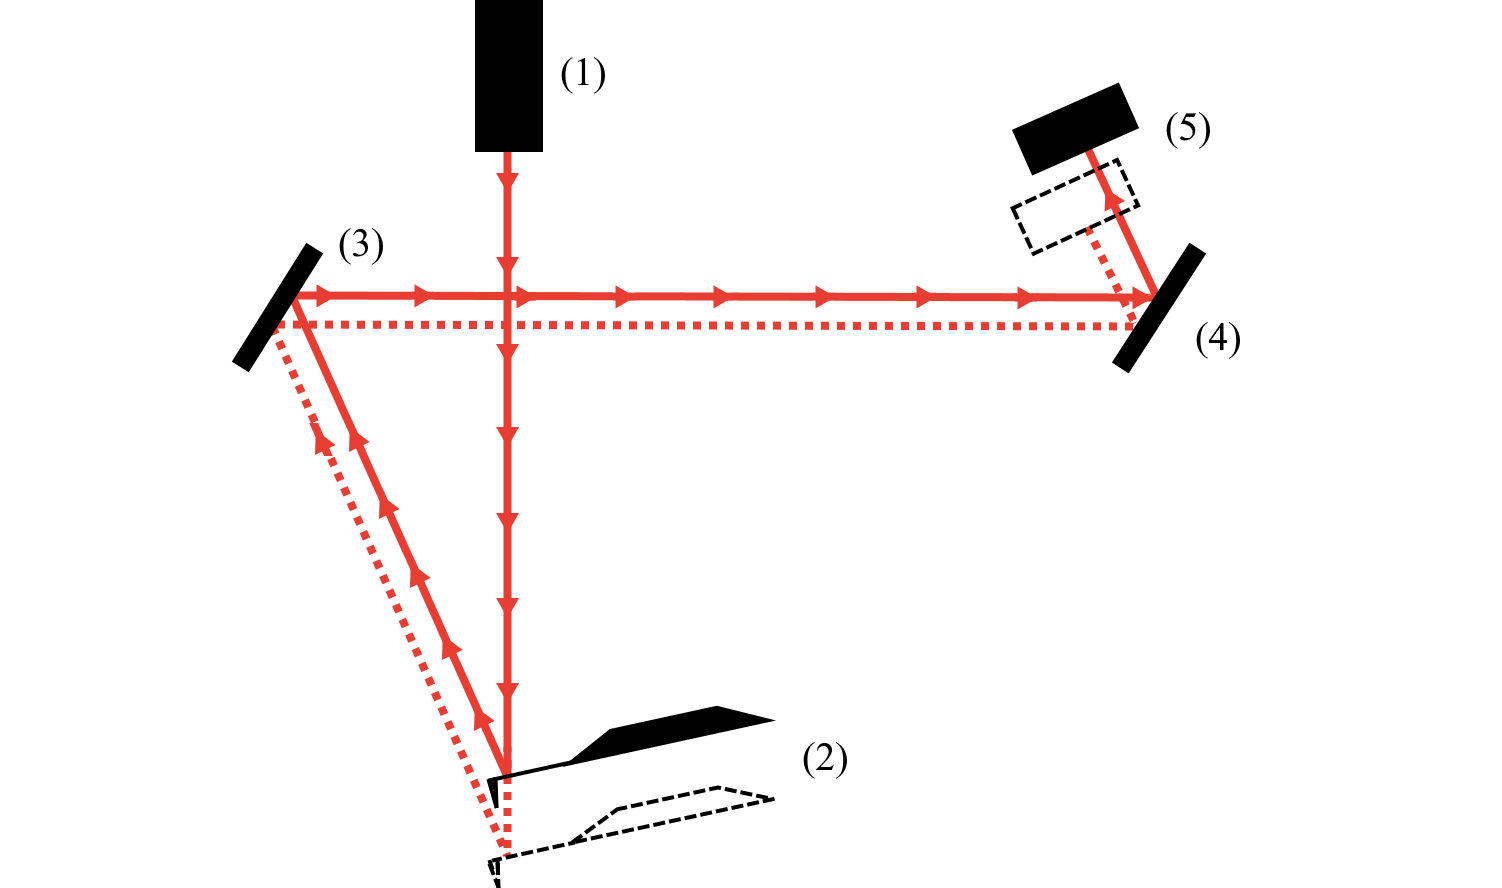
\includegraphics[width=1.0\linewidth]{afm_principles.png}
    \caption[Illustration of the principles behind \ac{afm}.]{Illustration of the principles behind \ac{afm}. The setup consists of: (1) laser, (2) cantilever with a sharp tip, (3) steering mirror, (4) stationary mirror, and (5) \acf{pspd}. The red line represents the laser beam and the dotted red line show how the path is changed by the deflection of the cantilever \citep[Adapted from][]{psia2002xe100}.}
    \label{fig:afm_laser}
\end{figure}

An \ac{afm} image is a convolution between the tip and the sample which is to be visualised. Therefore, the tip radius limits the lateral resolution, and cause an image artifact which is observable when using a tip with a similar or higher radius of curvature with respect to the feature. Holes can appear both narrower and less deep, and protruding features can appear wider than they really are, see Fig.~\ref{fig:afm_tip-convolution}. For the technique to provide information of the surface at the atomic level, the tip must be sharp, ideally terminating in just a single atom on the tip. Any changes to the tip that cause it to become broader, will decrease the lateral resolution of the image. These changes might be caused by contaminants on the tip or wearing of the tip due to collisions with the sample by either scanning too fast or having a rough surface \citep{birdi2003scanning}.

\begin{figure}[htbp]
    \centering
    \mySubfigure{0.49\linewidth}{afm_artifact_small-tip.png}[fig:afm_artifact_small]
    \hfill
    \mySubfigure{0.49\linewidth}{afm_artifact_big-tip.png}[fig:afm_artifact_large]
    \caption[Illustration of the convolution effect in an \ac{afm} image due to tip size.]{Illustration of an \ac{afm} image artifact that is caused by the convolution effect between the tip and the feature which is to be visualised, i.e. a broadening effect. This image artifact is observable when using a tip with \subref{fig:afm_artifact_small} a similar or \subref{fig:afm_artifact_large} higher radius of curvature with respect to the feature being imaged. In the images, grey represents the probe tip, black represents the real surface and surface features, and red represents the displayed surface \citep[Adapted from][]{psia2002xe100}.}
    \label{fig:afm_tip-convolution}
\end{figure}

\subsection{Surface Roughness}

Surface roughness is used as a quantitative measurement of surface changes. Surface roughness refers to height variations on the surface in the direction of the normal vector of a reference plane. There are many ways to characterise roughness, but one of the most commonly used for describing \ac{afm} images is the \ac{rms} roughness \citep{eaton2010atomic}. \Ac{rms} roughness is a statistical parameter given by \citep{thomas1999amplitude}
\begin{equation}\label{eq:rmsroughness}
R_\textrm{q} = \sqrt{\frac{1}{N}\sum_{i=1}^{N}\brackets{z_i-\bar{z}}^2},
\end{equation}
where $N$ is the number of data points in the image, $z_i$ is the height at point $i$, and $\bar{z}$ is the average elevation of the image profile. %reflects the roughness of the sample and is obtained by the Fourier Transform of the image.

%%=========================================
\section{Fourier Transform Infrared Spectroscopy}\label{sec:ftir}
\Acf{ftir} is a technique that is used to obtain an \ac{ir} transmission spectrum of a material. The spectrum indicates how much light that is transmitted through the sample at each wavelength. Patterns in the spectrum can help identify impurities and contaminants in the sample, since molecules exhibit specific \ac{ir} transmission fingerprints \citep{smith2011fourier}.

The transmittance spectrum, the percentage of incoming light that is transmitted through the sample as a function of wavenumber, is found by calculating the ratio of the sample spectrum and the background spectrum. The background spectrum is usually acquired immediately before the sample is placed in the sample compartment to get as identical conditions as possible.

\begin{figure}[htbp]
    \centering
    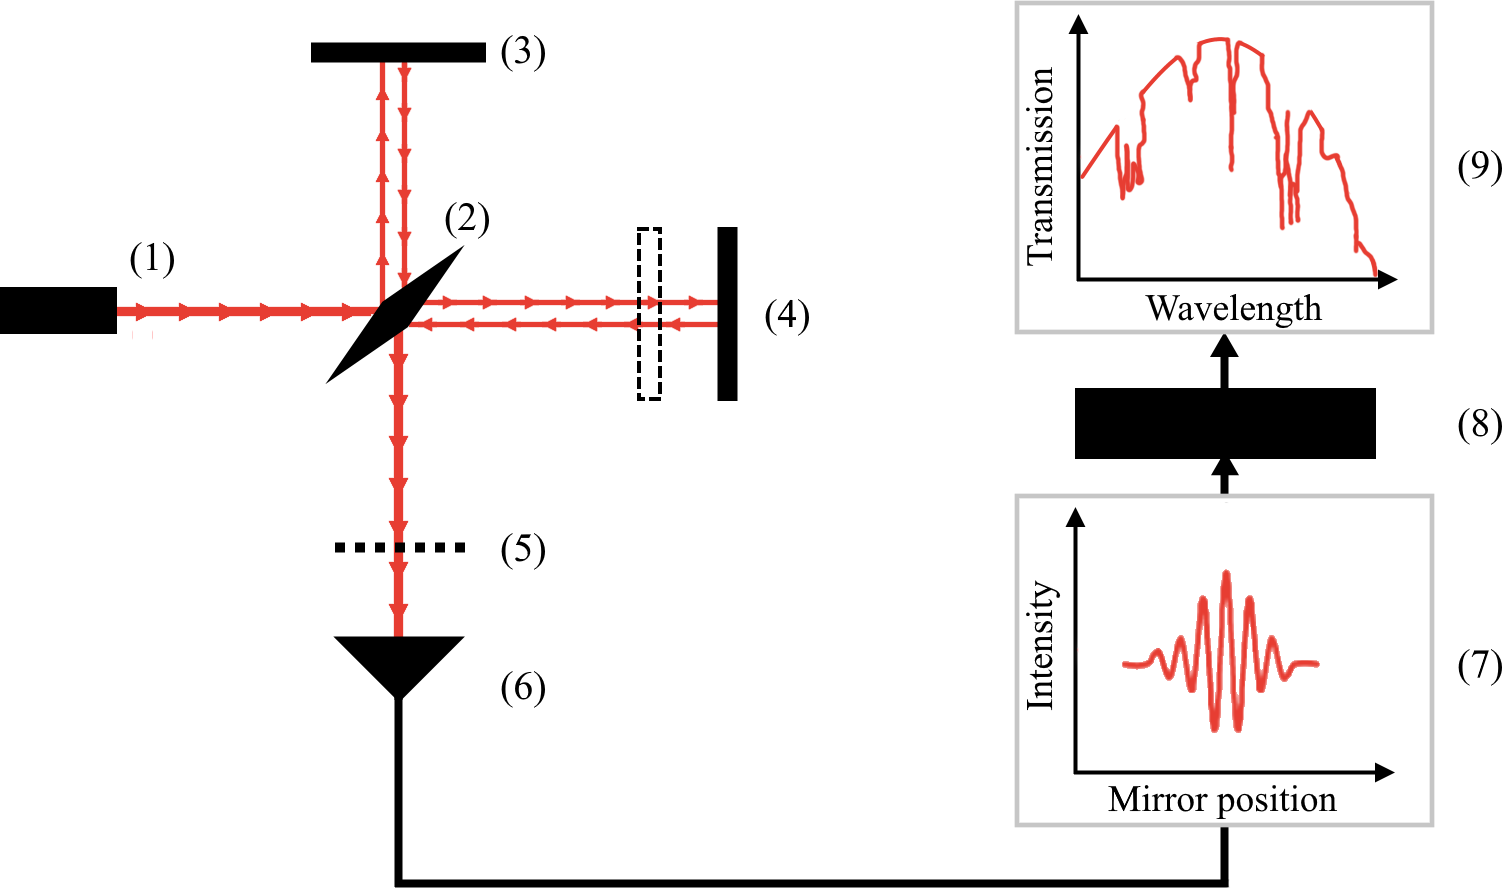
\includegraphics[width=1.0\linewidth]{ftir_principles.png}
    \caption[Illustration of the principles behind \ac{ftir}.]{Illustration of the principles behind \ac{ftir}. The setup consists of: (1) light source, (2) beamsplitter, (3) fixed mirror, (4) movable mirror, (5) sample compartment, (6) detector, (7) interferogram, (8) Fourier transform, and (9) \ac{ir} transmission spectrum \citep[Adapted from][]{nicolet2001introduction}.}% A beam of photons is first shone into a Michelson interferometer where the beamsplitter splits the light into two beams. One beam is refracted towards the fixed mirror and the other is transmitted towards the movable mirror. The beams are reflected back and combined at the beamsplitter. The resulting interference pattern is directed to the sample, and the detector measures how much of the beam that is transmitted through the sample as a function of mirror position, known as an interferogram. A Fourier transform is used to find how much each wavelength contributes to the signal, and convert the interferogram to a spectrum that show the intensity of the beam that is transmitted as a function of wavelength.}
    \label{fig:ftir_michelson}
\end{figure}

A beam of photons -- containing a range of wavelengths -- is first shone into a Michelson interferometer before it hits the sample. The Michelson interferometer contains a beamsplitter, which splits the light source into two. One beam is refracted towards a fixed mirror and the other is transmitted towards a movable mirror. The beams are reflected back towards the beamsplitter where they recombine, see Fig.~\ref{fig:ftir_michelson}. The difference in optical path length between the two beam paths, known as the \ac{opd}, is adjusted by moving the movable mirror. The resulting interference pattern is directed to the sample, and the detector measures how much of the beam that is transmitted through the sample as a function of mirror position, known as an interferogram.

As the mirror moves continuously from an \ac{opd} of zero to a distance further away, the intensity pattern of one specific wavelength $\lambda$ goes from constructive interference at \ac{opd}$=0$ to destructive interference where \ac{opd}$=(n+\frac{1}{2}) \lambda$ and constructive interference where \ac{opd}$= n \lambda$ for $n\in\mathbb{N}$. Waves which are not completely in or out of phase will have an intermediate intensity pattern. The interferogram is the sum of the interference patterns from all the different wavelengths measured at many discrete mirror positions. A Fourier transform is used to find how much each wavelength contributes to the signal, and converts the interferogram to a spectrum that shows the intensity of the beam that is transmitted as a function of wavelength \citep{smith2011fourier}.

%Since the Michelson interferometer has only a finite maximum \ac{opd}, it do not meet the requirements of the Fourier transform that the interferogram should be integrated from $-\infty$ to $+\infty$ \citep{bretzlaff1986apodization}.
%A problem that is encountered while doing 
%
%The resolution of the spectrum is set by the range of the mirror
%
The band gap of a material can be determined from the \ac{ftir} spectrum as the wavelength where the transmission increases steeply with increasing wavelength. The increase in transmission occurs because the photons with energy greater than the band gap can be absorbed by the creation of an electron-hole pair, while photons with energy less than the band gap cannot and are transmitted.

The thickness of a thin layer on top of another material can be calculated from the \ac{ftir} spectrum. Both the surface of the layer and the boundary between the layer and the underlying material reflect the incoming beam of photons. This difference in optical path length cause constructive and destructive interference of the light, which manifests as a fringing effect in the \ac{ftir} spectrum. The maxima are found where the optical path difference equals an even number of wavelengths. Hence, the fringes in the spectrum can be used to determine the thickness of the film
\begin{equation}
\label{eq:ftir_thickness}
d = \frac{1}{2}\frac{1}{n\Delta k},
\end{equation}
where $n$ is the refractive index and $\Delta k$ is the average period for one fringe \citep{griffiths2007fourier, stuart2008modern}.
%
%%=========================================
